\section{相关求解算法简介及其实现}

\subsection{MGDN}

文章提出一种跨域图表示学习方法。
核心思想是通过构建多域图结构,将不同域的行为特征统一编码。
该方法结合不同域的数据,利用注意力机制图卷积网络(Graph Convolutional Networks,GCN)\cite{kipf2017semi}学习共享与域特定特征。
模型框架如\cref{figure:跨域表示学习的总体框架}所示。

\begin{figure}[ht]
    \centering
    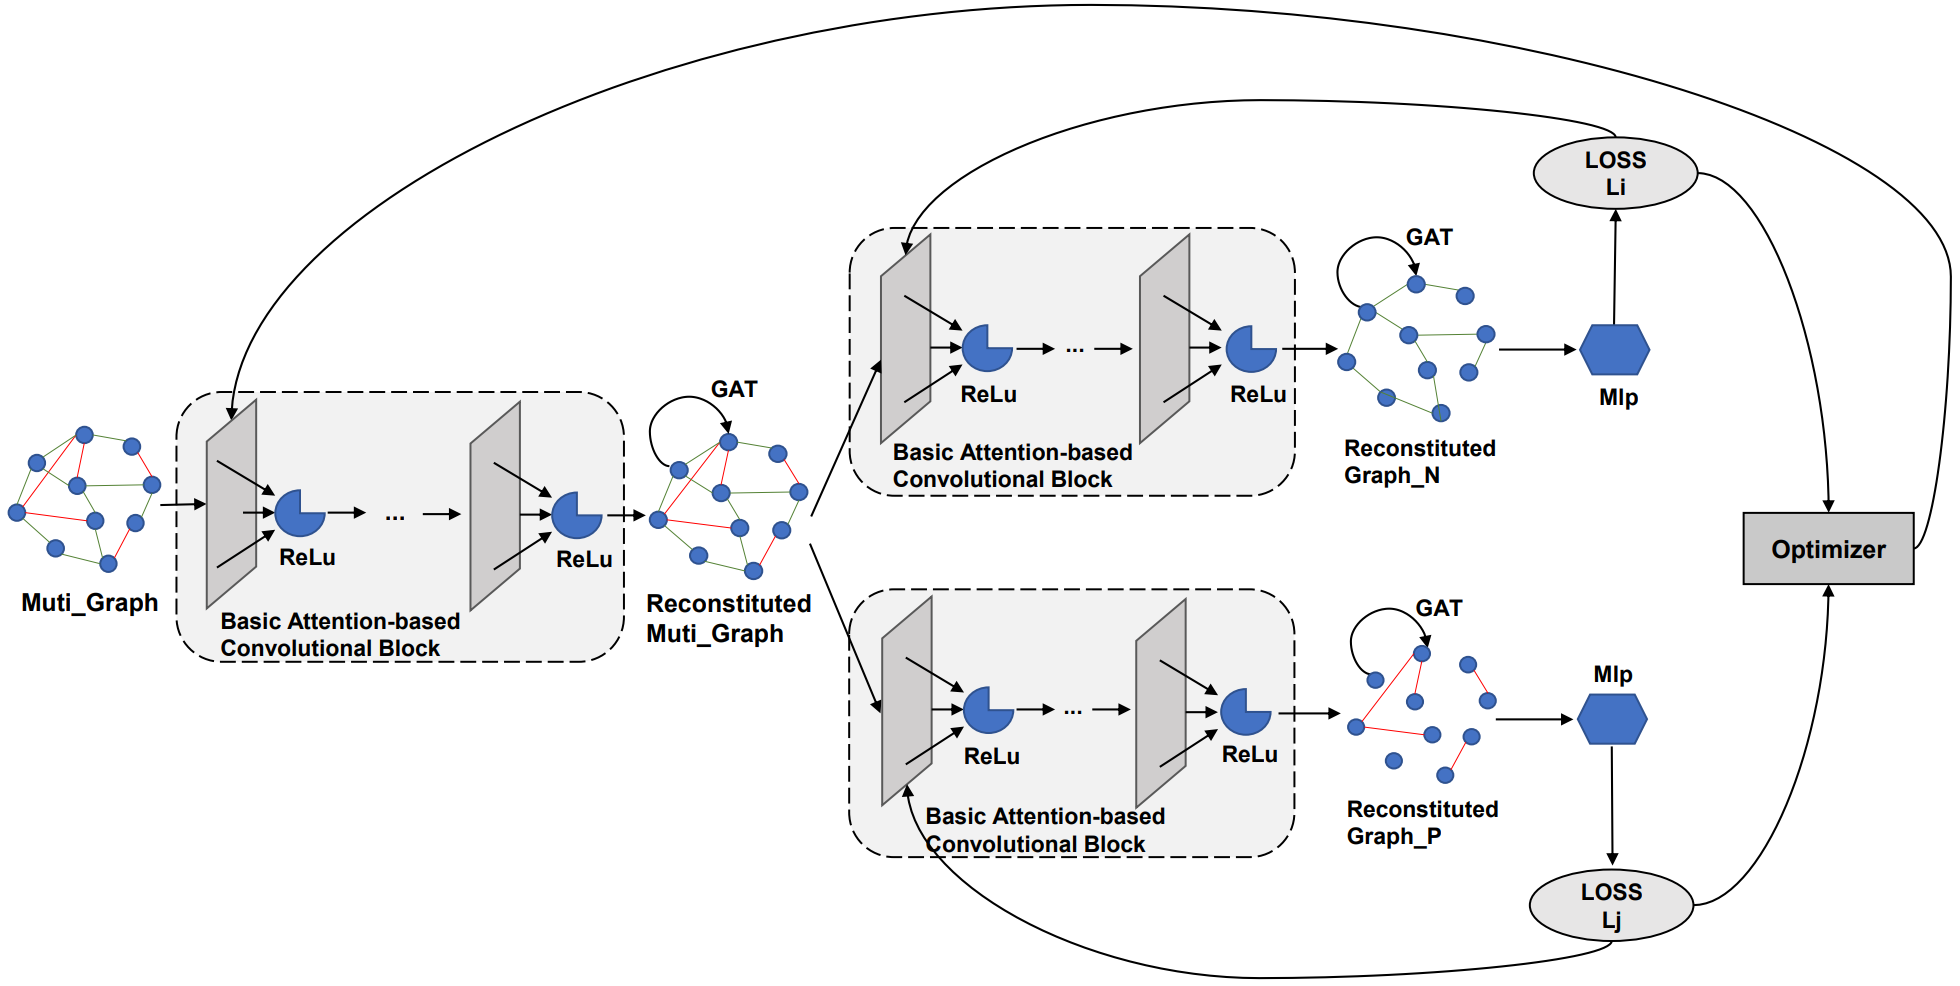
\includegraphics[width=1\textwidth]{img/跨域表示学习的总体框架.png}
    \caption{跨域表示学习的总体框架}
    \label{figure:跨域表示学习的总体框架}
\end{figure}

\subsubsection{多图构建}

在该方法中,目标是从ICS的多个域(如物理域、网络域等)中提取节点特征,并构建统一的多图结构用于跨域建模。
多图表示结构的构构建过程如\cref{figure:多图表示结构的构建过程}所示。

\begin{figure}[ht]
    \centering
    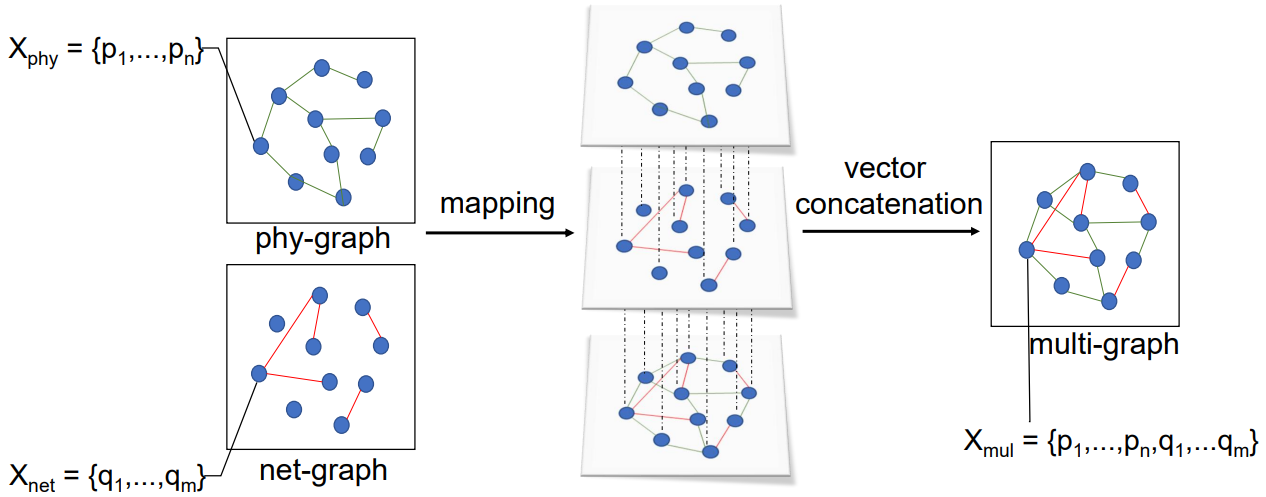
\includegraphics[width=1\textwidth]{img/多图表示结构的构建过程.png}
    \caption{多图表示结构的构建过程}
    \label{figure:多图表示结构的构建过程}
\end{figure}

假设有$n$个节点(传感器和执行器),来自不同域的数据被统一为相同的时间粒度(如秒级粒度),每个节点在第$d$个域上的特征矩阵为
\begin{equation*}
    \bm{x}^{(d)}\in\mathbb{R}^{n\times t} \text{,}
\end{equation*}
其中$t$为时间步长。

对每个域$d\in\{1,2,\cdots,D\}$, 构建一个无向加权图
\begin{equation*}
    \mathcal{G}_d=\left<\mathcal{V},\mathcal{E}_d\right> \text{,}
\end{equation*}
其中$\mathcal{V}$表示所有节点的集合,且$|\mathcal{V}|=n$,$\mathcal{E}_d$为第$d$个域中的边集合。

节点之间的边权通过余弦相似度计算其嵌入向量之间的相似性。
对于任意两个节点$i$和节点$j$,在第$d$域的嵌入向量为$\bm{v}_i^{(d)}$和$\bm{v}_j^{(d)}$,则计算节点$i$到节点$j$的边权
\begin{equation*}
    e_{ij}^{(d)}=\frac{\left(\bm{v}_i^{(d)}\right)^\mathrm{T}\bm{v}_j^{(d)}}{\left\|\bm{v}_i^{(d)}\right\|\left\|\bm{v}_j^{(d)}\right\|} \text{,}
\end{equation*}
之后使用Top-k策略筛选每个节点最相关的$k$个邻居构建图$\mathcal{G}_d$,进一步融合成多图结构
\begin{equation*}
    \mathcal{G}=\left<\mathcal{V}, \textstyle\bigcup_{i=1}^d\mathcal{E}_i\right> \text{,}
\end{equation*}
节点$i$的跨域特征向量表示为
\begin{equation*}
    \bm{v}_i=\bm{v}_i^{(1)}\oplus\bm{v}_i^{(2)}\oplus\cdots\oplus\bm{v}_i^{(D)} \text{。}
\end{equation*}

\subsubsection{基于注意力的图卷积建模}

该部分通过引入图注意力机制(Graph Attention Network, GAT)\cite{deng2021graph}对节点信息进行聚合,捕捉局部邻居中的非均匀关系。

首先,定义节点$j$对节点$i$的注意力权重
\begin{equation*}
    \alpha_{ij}=\mathrm{Softmax}\left(\mathrm{LeakeyReLU}\left(\bm{a}^\mathrm{T}(\bm{v}_i\oplus\bm{v}_j)\right)\right) \text{,}
\end{equation*}
其中$\bm{a}$为可学习的向量。则节点$i$的表示更新为
\begin{equation*}
    \bm{z}_i=\mathrm{ReLU}\left(\alpha_{ii}\bm{W}\bm{v}_i+\bm{W}\sum_{j\in\mathcal{N}_i}\alpha_{ij}\bm{v}_j\right) \text{,}
\end{equation*}
其中$\bm{W}$为可学习的矩阵。

使用节点的聚合表示和特征向量进行输出,即
\begin{equation*}
    \hat{\bm{y}}=f_\theta([\bm{z}_1\circ\bm{v}_1, \bm{z}_2\circ\bm{v}_2, \cdots, \bm{z}_n\circ\bm{v}_n]) \text{,}
\end{equation*}
其中$\circ$为逐元素乘法,$f_\theta$为多层感知机。


\subsubsection{多目标优化}

为了在多个域(如物理域、网络域等)上同时优化预测性能,文章使用了多任务学习(Multi-Task Learning, MTL)方法,其目标是联合优化每个任务的损失
\begin{equation*}
    \min_{\bm{W}_s,\bm{W}_1,\bm{W}_2,\cdots,\bm{W}_D}\sum_{d=1}^D\gamma_d\mathcal{L}_d(\bm{W}_s,\bm{W}_d) \text{,}
\end{equation*}
其中$\bm{W}_s$为共享层参数,$\bm{W}_d$、$\mathcal{L}_d$和$\gamma_d$分别为第$d$域的专属参数、损失函数及任务权重。

为了解决梯度冲突问题,引入了多梯度下降算法(Multiple Gradient Descent Algorithm,MGDA)\cite{desideri2012multiple},其基本思想是寻找一组权重$\{\gamma_d\}$,使得多个损失函数在共享参数$\bm{W}_s$上的梯度方向可以共同优化,即
\optmodule{\min_{\gamma_1,\gamma_2,\cdots,\gamma_D}}{\left\|\sum_{d=1}^D\gamma_d\nabla_{\bm{W}_s}\mathcal{L}_d(\bm{W}_s,\bm{W}_d)\right\|^2}{
    &\sum_{d=1}^D\gamma_d=1\text{,} \\
    &\gamma_1,\gamma_2,\cdots,\gamma_D\geq0\text{,}
    \label{equation:MGDA}
}
该优化问题保证在共享参数更新中不会偏向某一特定任务。

文章中的$D=2$,因此\cref{equation:MGDA}可简化为
\optmodule*{\min_{\gamma}}{\left\|\gamma\nabla_{\bm{W}_s}\mathcal{L}_1(\bm{W}_s,\bm{W}_1)+(1-\gamma)\nabla_{\bm{W}_s}\mathcal{L}_2(\bm{W}_s,\bm{W}_2)\right\|^2}{
    &\gamma\geq0\text{。}
}

\subsection{MicroDig}

为了捕捉性能问题的传播模式并进一步缩小候选根本原因的范围,文章对关联图中的每一条边执行异常检测,使用一种高效且广泛使用的异常检测方法——$k$-$\sigma$方法。
该方法从历史数据中学习参数$\mu$和$\sigma$,并将超出$(\mu-k\sigma,\mu+k\sigma)$范围的值视为异常。

文章基于端口级数据进行异常检测,而不是基于服务级数据,因为端口级的异常可能意味着包含该端口的服务存在异常行为,如果基于从端口级数据汇总的服务级数据进行异常检测,可能会被这些异常淹没。
根据上述步骤,文章保留了关联图中存在异常的边。
由于通过上述步骤得到的图是端口级关联图,而文章的目标是定位异常服务,因此需要合并端口的调用数据,并构建服务级关联图。

令$p$为端口级关联图中的一个节点,用$P(S)$表示给定服务$S$的所有端口。
为了构建服务级图,需要将同一服务$S$的所有端口级节点合并为一个节点,记为$S = \{p\in P(S)\}$。在服务级图上,边$S\to^{call}S'$的异常率$R(S, S')$整合了每个相关端口级边$p\to^{call}p'$的异常调用数$F(p, p')$和总调用数$N(p, p')$,即对于时间节点$t$,有
\begin{equation*}
    R_t(S, S')=\frac{\displaystyle\sum_{p\in S,p'\in S'}F_t(p,p')}{\displaystyle\sum_{p\in S,p'\in S'}N_t(p,p')}
\end{equation*}

通过上述步骤,可以构建一个服务级关联图,其中的节点都与问题服务相关。
同时,可以获得边$S = \{p\in P(S)\}$的异常率时间序列:
\begin{equation*}
    R(S,S')=(R_{t-\varphi},R_{t-\varphi+1},\cdots,R_{t+\varphi})
\end{equation*}
该时间序列表示在时间区间$[t-\varphi,t+\varphi]$之间中边$S\to^{call}S'$的异常率变化。
MicroDig的总体框架如\cref{figure:MicroDig的总体框架}所示。

\begin{figure}[ht]
    \centering
    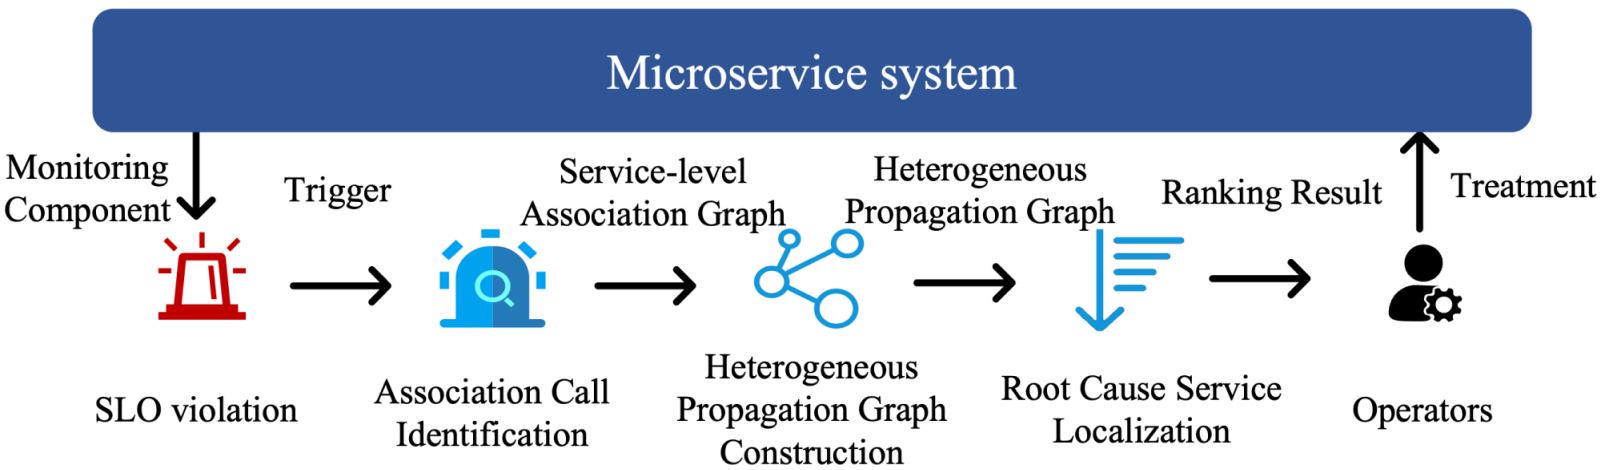
\includegraphics[width=\textwidth]{img/MicroDig框架.png}
    \caption{MicroDig的总体框架}
    \label{figure:MicroDig的总体框架}
\end{figure}

\subsubsection{异构传播图的构造}

构建的关联图是有向图,其边的方向表示服务之间的调用关系。
然而,调用关系并不等同于因果关系。
因此,关联图不能直接用作根本原因定位的因果图。
文章提出构建一个异构传播图,以反映调用和服务之间的因果关系,基于关联图进行构建。

\begin{algorithm}[!ht]
    \caption{异构传播图构造}
    \label{alg:Heterogeneous Propagation Graph Construction}
    \begin{algorithmic}[1]
        \State$G_h$\Get 初始化异构传播图
        \State$G_h$.addNodes($G$.edges())

        \ForAll{$S\in G$.nodes()}
            \ForAll{$C_{out}\in G$.outEdges($S$)}
                \ForAll{$C_{in}\in G$.inEdges($S$)}
                    \State $G_h$.addEdge($C_{out}$, $C_{in}$)
                \EndFor
            \EndFor
        \EndFor

        \State $G_h$.addNodes($G$.nodes())
        \ForAll{$C\in G$.edges()}
            \State $caller$, $callee$\Get\Call{splitCall}{$C$}
            \State $G_h$.addEdge($caller$, $C$)
            \State $G_h$.addEdge($callee$, $C$)
        \EndFor
    \end{algorithmic}
\end{algorithm}

\subsubsection{根因定位}

为了在异构传播图中进行根因定位,文章提出了一种新颖的方法,称为异构导向随机游走(Heterogeneity-Oriented Random Walk, HORW)。
该方法充分考虑了异构性的特点,并在转移概率的计算上进行了创新。
HORW方法的核心思想是通过模拟在异构传播图中的随机游走过程来识别根本原因。
与传统的随机游走方法不同,HORW不仅考虑了图中的节点和边的结构信息,还结合了不同类型的节点(如服务节点、调用节点)和边(如服务间调用、调用节点之间的因果关系)的异构特性。
通过对每种类型的边和节点赋予不同的权重,HORW能够更加精确地捕捉性能问题的传播路径,从而准确定位到根本原因服务。
该方法的创新之处在于转移概率的计算,即根据图中节点的类型和关联的边的性质来调整转移概率,而不是简单地依赖于图的结构。
这使得HORW能够更有效地识别和定位性能问题的根源,尤其是在复杂和动态的微服务环境中。
